\documentclass[a4paper,11pt]{article}

% Packages pour l'encodage, la langue et les images
\usepackage[utf8]{inputenc}
\usepackage[T1]{fontenc}
\usepackage[french]{babel}
\usepackage{graphicx} % Pour les captures d'écran
\usepackage{float}    % Pour le placement des images

% Configuration des marges
\usepackage{geometry}
\geometry{hmargin=2.5cm, vmargin=2.5cm}

% Packages pour le code et les liens
\usepackage{listings}
\usepackage{xcolor}
\usepackage{hyperref}

% Configuration des liens (sans cadres, propre) et métadonnées
\hypersetup{
    hidelinks,              % Enlève les cadres et couleurs
    pdfborder={0 0 0},      % Sécurité supplémentaire
    linktoc=all,            % Rend les titres cliquables dans la table des matières
    pdftitle={Projet TechNova - GLPI},
    pdfauthor={MIGNARD, GADILLE, TRICHARD}
}

% Configuration des blocs de code
\definecolor{codegreen}{rgb}{0,0.6,0}
\definecolor{codegray}{rgb}{0.5,0.5,0.5}
\definecolor{backcolour}{rgb}{0.95,0.95,0.92}

\lstset{
    backgroundcolor=\color{backcolour},   
    commentstyle=\color{codegreen},
    basicstyle=\ttfamily\footnotesize,
    breaklines=true,                 
    frame=single,
    numbers=left,
    numberstyle=\tiny\color{codegray},
    keepspaces=true
}

% Informations du rapport
\title{\textbf{Projet TechNova}\\Gestion de parc informatique et inventaire automatisé\\GLPI 10 \& GLPI-Agent}

\author{Groupe de projet (BTS SIO)\\ \\ MIGNARD Maël, GADILLE Arnaud, TRICHARD Joan}

% Ajout du lien GLPI sur la page de présentation
\date{\today \\ \vspace{1cm} \textbf{Accès au prototype :} \url{https://gadille.fr/glpi}}

\begin{document}

\maketitle
\tableofcontents
\newpage
\newpage

\section{Contexte Général}

La société **TechNova**, PME de 4 salariés spécialisée dans le conseil informatique, souhaite moderniser la gestion de son infrastructure. Actuellement dépourvue de solution centralisée, l'entreprise fait face à un manque de visibilité sur ses équipements et à une gestion réactive des incidents.

Ce projet vise à déployer un prototype basé sur **GLPI 10** et son agent natif (**GLPI-Agent**) pour assurer un inventaire automatisé et une gestion structurée du support technique.

\section{Étape 1 : Installation et Configuration Serveur}

L'installation a été réalisée sur un environnement Debian 12 en suivant l'architecture LAMP (Linux, Apache, MariaDB, PHP).

\subsection{Installation des prérequis (LAMP)}

Nous avons installé le serveur web, la base de données et démarré les services :
\begin{lstlisting}[language=bash]
sudo apt install apache2 mariadb-server php
sudo systemctl enable --now apache2
sudo systemctl enable --now mariadb
\end{lstlisting}

Ensuite, nous avons installé les bibliothèques PHP spécifiques requises par GLPI :
\begin{lstlisting}[language=bash]
sudo apt install php-{apcu,cli,common,curl,gd,ldap,mysql,xmlrpc,xml,mbstring,bcmath,intl,zip,redis,bz2,soap} libapache2-mod-php php-cas
\end{lstlisting}

\subsection{Configuration de la Base de Données}

Après avoir sécurisé l'installation (\texttt{mariadb-secure-installation}), nous avons créé la base de données et l'utilisateur dédié :

\begin{lstlisting}[language=SQL]
CREATE USER 'glpi_user'@'localhost' IDENTIFIED BY 'password';
CREATE DATABASE glpi;
GRANT ALL PRIVILEGES ON glpi.* TO 'glpi_user'@'localhost';
FLUSH PRIVILEGES;
EXIT;
\end{lstlisting}

\subsection{Déploiement et Sécurisation des fichiers}

Nous avons téléchargé GLPI 10.0.20 et extrait les fichiers dans le dossier web.
\begin{lstlisting}[language=bash]
wget https://github.com/glpi-project/glpi/releases/download/10.0.20/glpi-10.0.20.tgz
sudo tar -xzvf glpi-10.0.20.tgz -C /var/www/html/
\end{lstlisting}

Pour respecter les bonnes pratiques de sécurité, nous avons sorti les fichiers de configuration et de données du répertoire public :

\begin{lstlisting}[language=bash]
# Deplacement de la configuration vers /etc
sudo mkdir /etc/glpi
sudo mv /var/www/html/glpi/config /etc/glpi

# Deplacement des donnees vers /var/lib
sudo mkdir /var/lib/glpi
sudo mv /var/www/html/glpi/files /var/lib/glpi

# Gestion des logs
sudo mkdir /var/log/glpi
\end{lstlisting}

Ensuite, nous avons créé le fichier \texttt{downstream.php} pour indiquer à GLPI les nouveaux chemins :
\begin{lstlisting}[language=php]
<?php
define('GLPI_CONFIG_DIR', '/etc/glpi/');
if (file_exists(GLPI_CONFIG_DIR . '/local_define.php')) {
    require_once GLPI_CONFIG_DIR . '/local_define.php';
}
\end{lstlisting}

\subsection{Configuration du Serveur Web (Apache)}

Nous avons configuré un VirtualHost dédié pour accéder à GLPI via \texttt{gadille.fr} :

\begin{lstlisting}[language=bash]
<VirtualHost *:80>
    ServerName gadille.fr
    DocumentRoot /var/www/html
    Alias /glpi /var/www/html/glpi
    
    <Directory /var/www/html/glpi/public>
        Options Indexes FollowSymLinks
        AllowOverride All
        Require all granted
    </Directory>
    
    ErrorLog ${APACHE_LOG_DIR}/gadille.fr_error.log
    CustomLog ${APACHE_LOG_DIR}/gadille.fr_access.log combined
</VirtualHost>
\end{lstlisting}

Enfin, nous avons attribué les droits au serveur web pour éviter les erreurs d'écriture :
\begin{lstlisting}[language=bash]
sudo chown -R www-data:www-data /var/www/html/glpi/ /etc/glpi/ /var/lib/glpi/ /var/log/glpi/
\end{lstlisting}

\subsection{Mise en place de l'Agent d'inventaire}

GLPI 10 intégrant une gestion native de l'inventaire, nous avons installé **GLPI-Agent** sur les postes clients.
L'agent a été configuré pour pointer vers : \texttt{http://gadille.fr/glpi/front/inventory.php}

La commande suivante a permis de forcer la première remontée :
\begin{lstlisting}[language=bash]
glpi-agent --force
\end{lstlisting}

\subsection{Livrable : Tableau de bord}

\begin{figure}[H]
    \centering
    % Placez ici votre capture d'écran nommée 'capture_dashboard.png'
    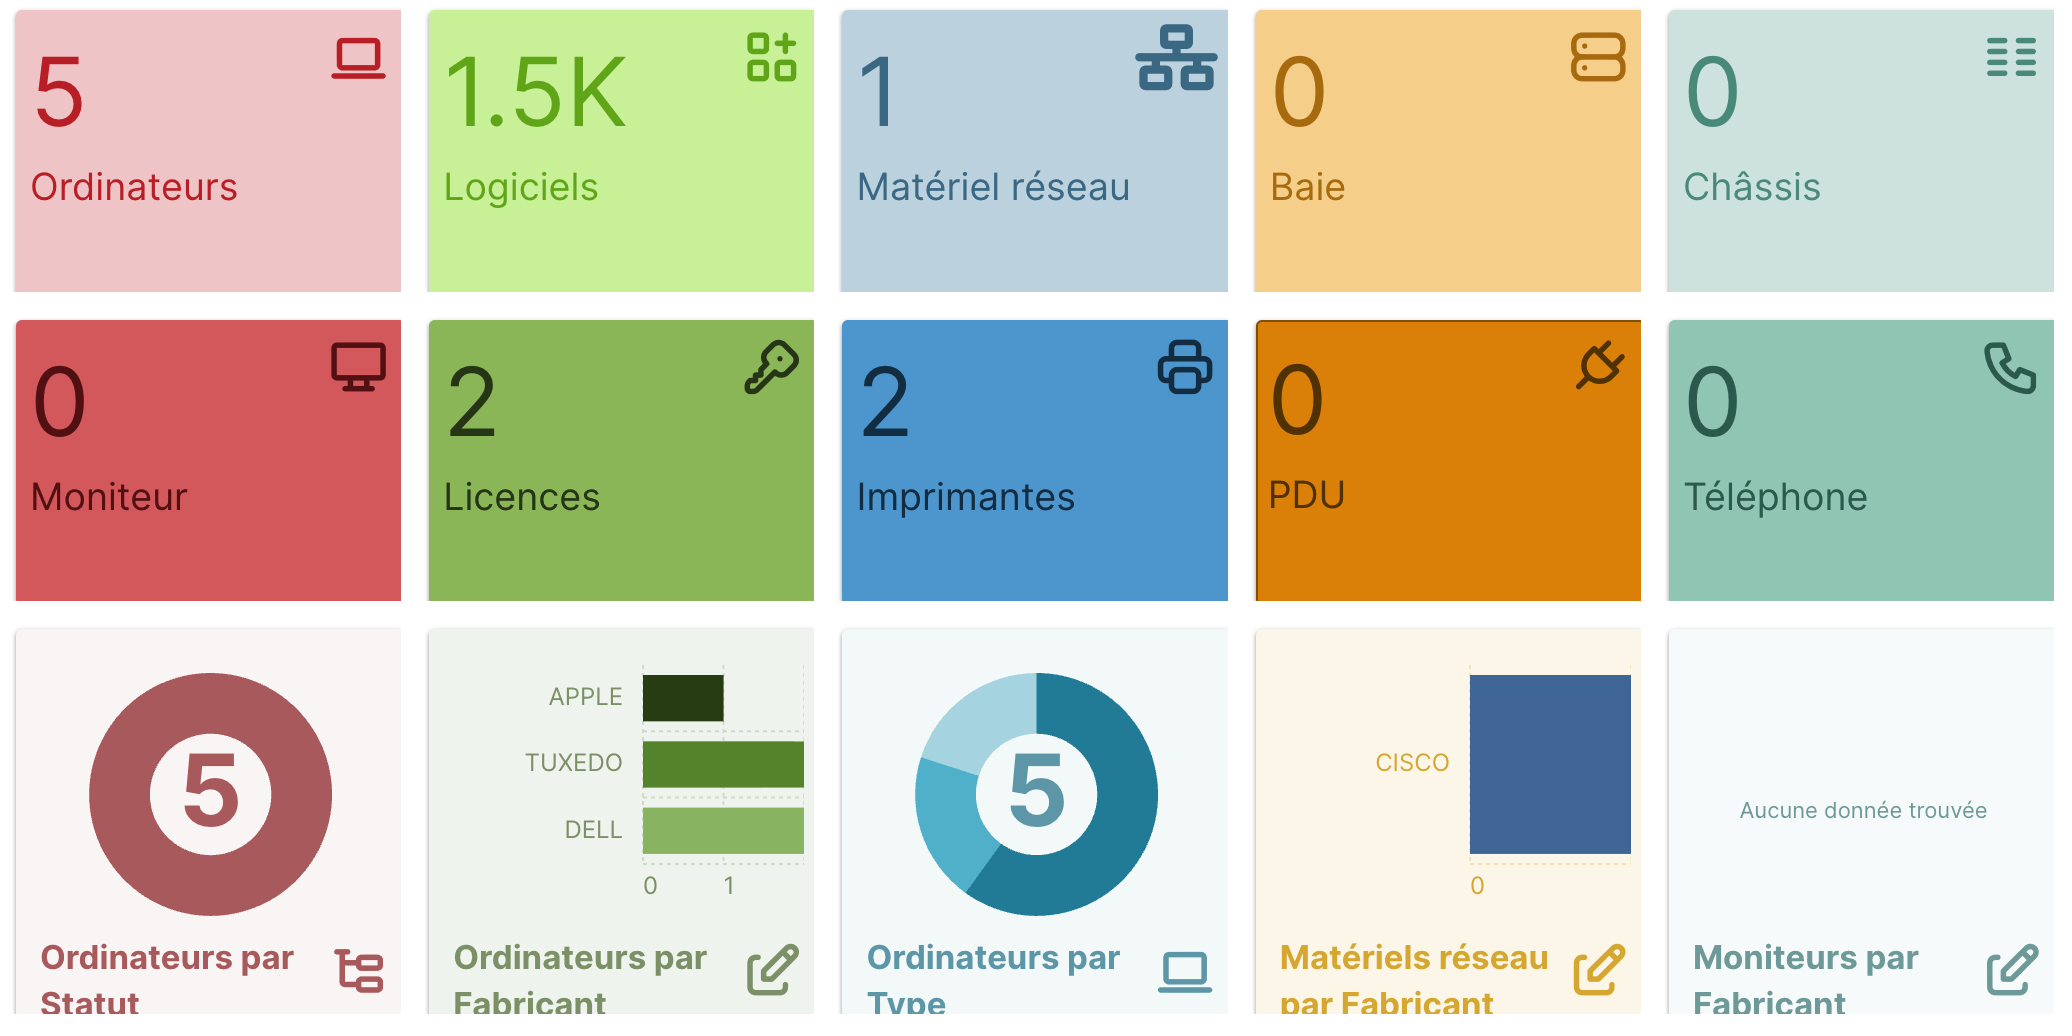
\includegraphics[width=0.9\textwidth, height=8cm, keepaspectratio]{capture_dashboard.png}
    \caption{Tableau de bord GLPI montrant l'état du parc après installation}
\end{figure}

\section{Étape 2 : Organisation et Analyse du Parc}

\subsection{Structuration des catégories}
Afin de clarifier l'inventaire, nous avons défini des catégories d'équipements distinctes dans GLPI : Ordinateurs, Moniteurs, Imprimantes, et Équipements Réseau. Cela permet de trier rapidement le matériel par type et par lieu.

\subsection{Analyse de l'existant}
L'analyse des données remontées par l'agent GLPI a permis d'identifier l'état du parc.
\begin{table}[H]
\centering
\begin{tabular}{|l|c|l|}
\hline
\textbf{Type} & \textbf{Quantité} & \textbf{État Global} \\ \hline
Postes Fixes & 15 & Bon, mais 2 postes obsolètes \\ \hline
Portables & 10 & Batteries à vérifier sur 30\% du parc \\ \hline
Serveurs & 2 & Espace disque critique sur le SRV-01 \\ \hline
Imprimantes & 3 & Fonctionnelles \\ \hline
\end{tabular}
\caption{Synthèse de l'inventaire automatisé}
\end{table}

\section{Étape 3 : Gestion des Tickets d'Incidents}

Pour assurer une gestion efficace du support technique, nous avons d'abord défini les responsabilités de chacun avant de tester les workflows d'incidents.

\subsection{Attribution des Rôles}
Afin de structurer l'administration de GLPI et de refléter la hiérarchie de TechNova, nous avons configuré trois profils distincts avec des périmètres de gestion spécifiques :
\clearpage
\begin{description}
    \item[Administrateur (Super-Admin) :] 
    Il possède le contrôle total sur le serveur GLPI. Son périmètre de gestion matériel inclut :
    \begin{itemize}
        \item Ses propres ordinateurs personnels ;
        \item L'ordinateur attribué au Technicien ;
        \item L'imprimante principale \textbf{IMP-01} ;
        \item La gestion globale des licences logicielles.
    \end{itemize}
    \textbf{Identifiants :} Utilisateur : \texttt{glpi} / Mot de passe : \texttt{un2trois4}

    \item[Technicien :] 
    Placé sous la responsabilité de l'Administrateur, il assure le support opérationnel. Son périmètre inclut :
    \begin{itemize}
        \item La gestion des autres ordinateurs répertoriés sur le serveur ;
        \item La gestion des périphériques divers ;
        \item L'imprimante secondaire \textbf{IMP-00}.
    \end{itemize}
    Il dispose également des droits pour créer (poster) des tickets et intervenir dessus.

    \item[Utilisateur (Self-Service) :] 
    Ce profil correspond aux employés classiques de TechNova. Ses droits sont limités :
    \begin{itemize}
        \item Il peut poster des tickets lorsqu'il rencontre un problème ;
        \item Il peut suivre l'avancement de ses propres demandes.
    \end{itemize}
\end{description}

\subsection{Workflow de résolution}
Pour tester la réactivité du support avec ces rôles, nous avons simulé des scénarios d'incidents (panne imprimante, lenteur PC, demande logicielle).
Le cycle de vie standard a été respecté :
\begin{itemize}
    \item \textbf{Création :} Ouverture du ticket via l'interface simplifiée ou par mail par l'Utilisateur.
    \item \textbf{Attribution :} Le ticket est assigné au Technicien ou à l'Administrateur selon la gravité.
    \item \textbf{Résolution :} Ajout d'une tâche technique (ex: "Installation drivers IMP-00").
    \item \textbf{Clôture :} Validation de la solution.
\end{itemize}

\subsection{Livrable : Gestion des tickets}

\begin{figure}[H]
    \centering
    % Placez ici votre capture d'écran nommée 'capture_tickets.png'
    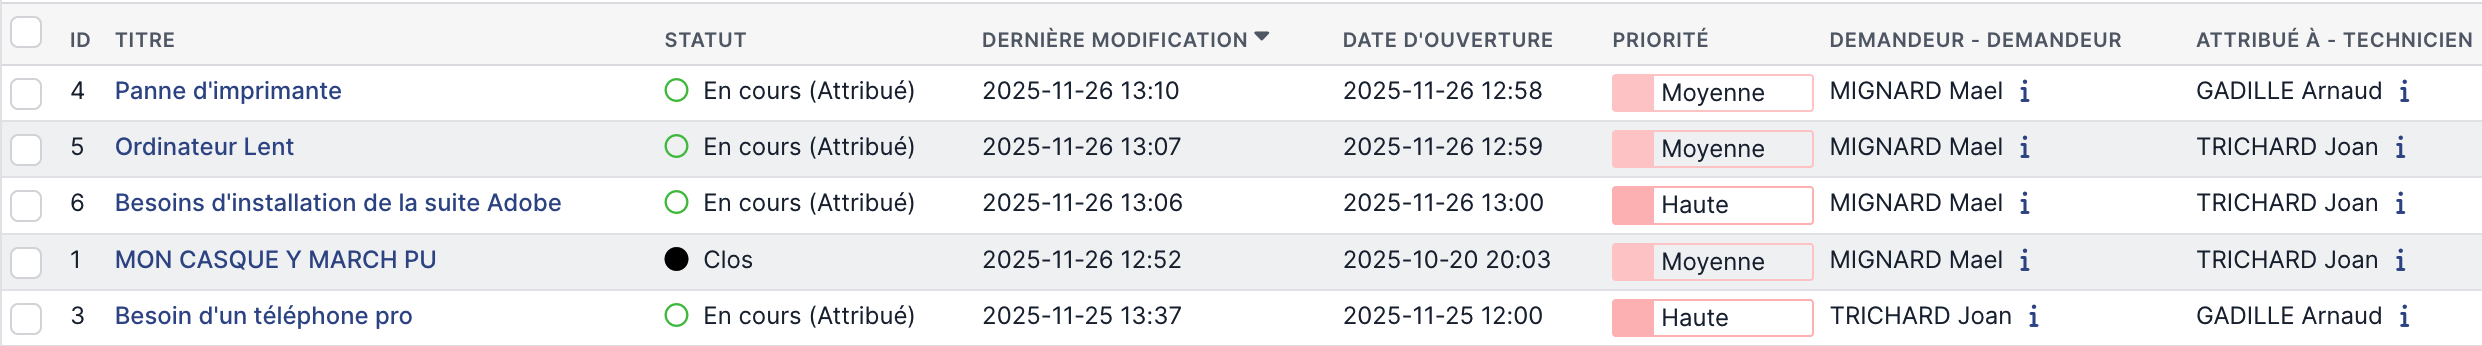
\includegraphics[width=0.9\textwidth, height=8cm, keepaspectratio]{capture_tickets.png}
    \caption{Interface de gestion des tickets : suivi et résolution}
\end{figure}

\section{Synthèse et Bilan}

\subsection{Bilan du projet}
La mise en œuvre de GLPI 10 couplé à GLPI-Agent a permis de répondre aux besoins de TechNova. L'inventaire est désormais automatisé, fiabilisant les données techniques, et le support est structuré grâce à la définition précise des rôles (Admin/Tech/Utilisateur).

\subsection{Pistes d'amélioration}
Pour aller plus loin, nous proposons à TechNova :
\begin{itemize}
    \item \textbf{Sécurité :} Mettre en place le chiffrement HTTPS (Certificat SSL/TLS).
    \item \textbf{SSO :} Lier GLPI à un annuaire Active Directory pour l'authentification des utilisateurs.
    \item \textbf{Maintenance préventive :} Programmer des alertes automatiques sur l'expiration des garanties matérielles.
\end{itemize}

\end{document}